%%%%%%%%%%%%%%%%%%%%%%%%%%%%%%%%%%%%%%%%%%%%%%%%%%%%%%%%%%%%%%%%%%
%%%%%%%% ICML 2014 EXAMPLE LATEX SUBMISSION FILE %%%%%%%%%%%%%%%%%
%%%%%%%%%%%%%%%%%%%%%%%%%%%%%%%%%%%%%%%%%%%%%%%%%%%%%%%%%%%%%%%%%%

% Use the following line _only_ if you're still using LaTeX 2.09.
%\documentstyle[icml2014,epsf,natbib]{article}
% If you rely on Latex2e packages, like most moden people use this:
\documentclass{article}

\usepackage{amsthm,amsmath,amsfonts,mathtools,custom_math}
%\usepackage{caption,sidecap}

% use Times
\usepackage{times}
% For figures
\usepackage{graphicx} % more modern
%\usepackage{epsfig} % less modern
\usepackage{subfigure} 

% For citations
\usepackage{natbib}

% For algorithms
\usepackage{algorithm}
\usepackage{algorithmic}

% As of 2011, we use the hyperref package to produce hyperlinks in the
% resulting PDF.  If this breaks your system, please commend out the
% following usepackage line and replace \usepackage{icml2014} with
% \usepackage[nohyperref]{icml2014} above.
\usepackage{hyperref}

% Packages hyperref and algorithmic misbehave sometimes.  We can fix
% this with the following command.
\newcommand{\theHalgorithm}{\arabic{algorithm}}

% Employ the following version of the ``usepackage'' statement for
% submitting the draft version of the paper for review.  This will set
% the note in the first column to ``Under review.  Do not distribute.''
\usepackage{icml2014} 
% Employ this version of the ``usepackage'' statement after the paper has
% been accepted, when creating the final version.  This will set the
% note in the first column to ``Proceedings of the...''
%\usepackage[accepted]{icml2014}


% The \icmltitle you define below is probably too long as a header.
% Therefore, a short form for the running title is supplied here:
\icmltitlerunning{Variable Selection in Convex Function Estimation}


% ENVIRONMENTS
\numberwithin{equation}{section}
\theoremstyle{plain}
\newtheorem{theorem}{Theorem}[section]
\newtheorem{corollary}[theorem]{Corollary}
\newtheorem{proposition}[theorem]{Proposition}
\newtheorem{lemma}[theorem]{Lemma}
\newtheoremstyle{remark}{\topsep}{\topsep}%
     {\normalfont}% Body font
     {}           % Indent amount (empty = no indent, \parindent = para indent)
     {\bfseries}  % Thm head font
     {.}          % Punctuation after thm head
     {.5em}       % Space after thm head (\newline = linebreak)
     {\thmname{#1}\thmnumber{ #2}\thmnote{ #3}}% Thm head spec
\theoremstyle{remark}
\newtheorem{remark}[theorem]{Remark}
\newtheorem{example}[theorem]{Example}
\newtheorem{assumption}[theorem]{Assumption}
\newtheorem{definition}[theorem]{Definition}





\begin{document} 


% John's macros
\def\X{\mathcal{X}}
\def\comma{\unskip,~}
\def\truep{p^*}
\def\div{\|\,}
\long\def\comment#1{}
\def\reals{{\mathbb R}}
\def\P{{\mathbb P}}
\def\E{{\mathbb E}}
\def\Cov{\mathop{\text{Cov}}}
\def\supp{\mathop{\text{supp}\kern.2ex}}
\def\argmin{\mathop{\text{\rm arg\,min}}}
\def\arginf{\mathop{\text{\rm arg\,inf}}}
\def\argmax{\mathop{\text{\rm arg\,max}}}
\let\tilde\widetilde
\def\csd{${}^*$}
\def\mld{${}^\dag$}
\def\dos{${}^\ddag$}
\def\W{\widetilde Y}
\def\Z{\widetilde X}
\let\hat\widehat
\let\tilde\widetilde
\def\given{{\,|\,}}
\def\ds{\displaystyle}
\def\bs{\backslash}
\def\1{{(1)}}
\def\2{{(2)}}
\def\pn{{(n)}}
\def\ip{{(i)}}
\def\Xbar{\overline{X}}
\def\except{\backslash}
\def\npn{\mathop{\textit{NPN\,}}}
\def\i{{(i)}}
\def\cE{{\mathcal{C}}}
\def\cM{{\mathcal{M}}}
\def\cF{{\mathcal{F}}}
\def\cP{{\mathcal{P}}}
\def\cG{{\mathcal{G}}}
\def\tr{\mathop{\text{tr}}}
\long\def\comment#1{}
\def\ti#1{#1}
\def\titi#1{\textit{#1}}
\def\cram{{\sc cram}}
\def\spam{{\small\sc SpAM}}
\def\diag{\mathop{\rm diag}}
\def\ones{\mathbf{1}}
\def\threebars{\mbox{$|\kern-.25ex|\kern-.25ex|$}}
\def\fatnorm#1{\threebars #1 \threebars}
\def\rank{\mathop{\rm rank}}
\def\S{\mathcal{S}}
\def\H{\mathcal{H}}
\def\K{{K}}
\def\rank{\mathop{\rm rank}}
\def\half{{1/2}}
\def\Y{\mathbb{Y}}
\def\M{\mathbb{M}}
\def\F{\mathbb{F}}
\def\pinv{{-1}}
%\def\ones{\mathds{1}}
%\def\ones{1}
\def\Res{Z}
\def\Proj{P}
\def\cN{{\mathcal N}}
\def\cT{{\mathcal H}}
\def\coloneqq{:=}
\def\mathbf#1{\mbox{\boldmath $#1$}} 
\def\bar#1{\overline{#1}}




\twocolumn[
\icmltitle{Variable Selection in Convex Function Estimation}

% It is OKAY to include author information, even for blind
% submissions: the style file will automatically remove it for you
% unless you've provided the [accepted] option to the icml2014
% package.
\icmlauthor{Your Name}{email@yourdomain.edu}
\icmladdress{Your Fantastic Institute,
            314159 Pi St., Palo Alto, CA 94306 USA}
\icmlauthor{Your CoAuthor's Name}{email@coauthordomain.edu}
\icmladdress{Their Fantastic Institute,
            27182 Exp St., Toronto, ON M6H 2T1 CANADA}

% You may provide any keywords that you 
% find helpful for describing your paper; these are used to populate 
% the "keywords" metadata in the PDF but will not be shown in the document
\icmlkeywords{boring formatting information, machine learning, ICML}

\vskip 0.3in
]

\begin{abstract} 
  We consider the problem of estimating a sparse convex function of
  many variables.  In contrast to classical nonparametric
  regression with smoothness constraints, we show that convexity is
  additively faithful---it suffices to estimate a convex additive
  model for variable selection.  We develop algorithms for estimating
  sparse convex additive models, including an approach using iterative
  quadratic programming.  Supporting experiments and statistical
  theory are presented, showing variable selection consistency in
  dimensions that can scale exponentially in the sample size.  An
  attractive feature of this framework is the lack of tuning parameters
  for smoothness.
\end{abstract} 

\section{Introduction}


We consider the problem of estimating a convex function of several
variables from noisy values of the function at a finite sample of
input points.  Recent work \cite{Guntu:12,Guntu:13} shows that the
minimax rate for convex function estimation in $p$ dimensions is
$n^{-4/(4+p)}$.  Loosely speaking, this shows that the
geometric convexity constraint is statistically equivalent to
requiring two derivatives of the function, and thus is
subject to the same curse of dimensionality.
However, if the function is sparse, with $s\ll p$ relevant variables,
then the faster rate $n^{-4/(4+s)}$ may be achievable if the $s$
variables can be identified.  To determine the relevant variables, we
show that it suffices to estimate a sum of $p$ one-dimensional convex
functions, leading to significant computational and statistical
advantages.  In addition, we introduce algorithms and supporting
statistical theory for a practical, effective approach to this
variable selection problem.

The general sparse nonparametric regression problem is considered in \cite{lafferty2008rodeo}, where it is shown that computationally efficient, near minimax-optimal estimation is possible, but in ambient
dimensions that scale only as $p = O(\log n)$ instead of $p=O\bigl(e^{n^c}\bigr)$ as enjoyed by sparse linear models. \citet{dalalyan:12} do achieve exponential scaling $p=O(e^n)$ under certain Fourier smoothness conditions but they show that variable selection is still hard in that the number of relevant variables $s$ must be less than $\log n$.

% The general sparse nonparametric regression problem is considered in
% \cite{lafferty2008rodeo}, where it is shown that computationally
% efficient, near minimax-optimal estimation is possible, but in ambient
% dimensions that scale only as $p = O(\log n)$.  This is in stark
% contrast to the exponential scaling $p = O\bigl(e^{n^c}\bigr)$ enjoyed
% by sparse linear models \cite{Wain:09a}.  

Approximating the regression function by a sum of one-dimensional functions, known as sparse additive models, \cite{Ravikumar:09} is a practical alternative to fully
nonparametric function estimation.  But the additive assumption is
limited.  In particular, the natural idea of first selecting the
single variable effects, then the pairwise effects, and so on, does
not in general lead to consistent variable selection.  In other words,
the general nonparametric model is not additively faithful.
Remarkably, the additional assumption of convexity does lead to
consistent variable selection, as we show here. In addition, we show that
the scaling $p = O(\log n)$ and $n = O\big(\textrm{poly}(s)\big)$ is achievable for sparse convex additive models. Thus, the geometric convexity constraint is quite different from the
smoothness constraints imposed in traditional nonparametric
regression.

A key to our approach is the observation that least squares
nonparametric estimation under convexity constraints is equivalent to
a finite dimensional quadratic program.  Specifically, the infinite
dimensional optimization 
\begin{align}
\begin{split}
\text{minimize} & \quad \sum_{i=1}^n (Y_i - m(x_i))^2 \\
\text{subject to} &  \quad m:\reals^p\rightarrow\reals\ \text{is
  convex}
\end{split}
\end{align}
is precisely equivalent to the finite dimensional quadratic
program 
\begin{align}
\begin{split}
\label{eq:outer}
\text{minimize}_{h, \beta} & \;\; \sum_{i=1}^n (Y_i - h_i)^2 \\
\text{subject to} & \;\; h_j \geq h_i + \beta_i^T (x_j-x_i),\; \text{for
    all $i,j$}.
\end{split}
\end{align}
%\end{equation}
%See \cite{Boyd04}, Section 6.5.5.
Here $h_i$ is the estimated function value $m(x_i)$, and the vectors
$\beta_i \in \reals^d$ represent supporting hyperplanes to the
epigraph of $m$.  Importantly, this finite dimensional quadratic program does
not have tuning parameters for smoothing the function. Such parameters are the bane
of nonparametric estimation.

Estimation of convex functions arises naturally in several
applications.  Examples include geometric programming \cite{Boyd04},
computed tomography \cite{Prince:90}, target reconstruction
\cite{Lele:92}, image analysis \cite{Golden:06} and circuit design
\cite{Hannah:12}.  Other applications include queuing theory
\cite{Chen:01} and economics, where it is of interest to estimate
concave utility functions \cite{Pratt:68}.  See \cite{Lim:12} for
other applications.  

Beyond cases where the assumption of convexity is
natural, we offer that the convexity assumption is attractive as a
tractable, nonparamametric relaxation of the linear model.  In
addition to the lack of tuning parameters, other than the
regularization parameter $\lambda$ to control the level of sparsity,
the global convexity assumption leads to effective, scalable algorithms.  We
demonstrate use of our approach on experiments with standard
regression data sets, in a comparison with sparse linear models
(lasso).

%In the following section we give a high-level summary of our technical
%results, including additive faithfulness, variable selection 
%consistency, and high dimensional scaling.  In Section~X...

\def\mathbf#1{\mbox{\boldmath $#1$}} 


%\section{Related Work}
%\section{Summary of Results}
\section{Related Work}

\section{Additive Faithfulness}

For general regression, additive approximation may result in a
relevant variable being incorrectly marked as irrelevant. Such
mistakes are inherent to the approximation and may persist even with
infinite samples.  In this section we give
examples of this phenomenon, and then show how the convexity
assumption
changes the behavior of the additive approximation.  We begin
with a lemma that implies uniqueness of the additive regression function.


\begin{figure*}[htp]
\vskip-10pt
	\centering
	\subfigure[egg carton]{
		\centering
		{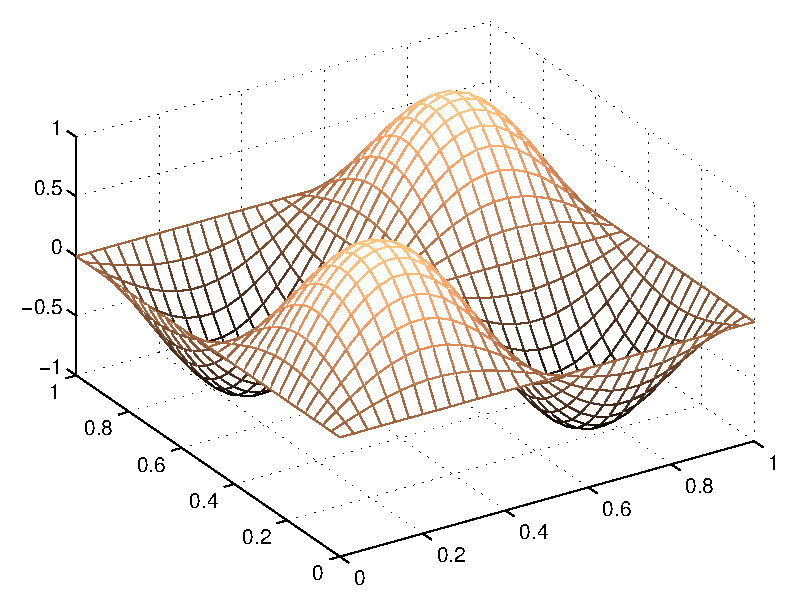
\includegraphics[width=0.4\textwidth]{../figs/sine_wave_funct3}}
	}
	\subfigure[tilting slope]{
		\centering
		{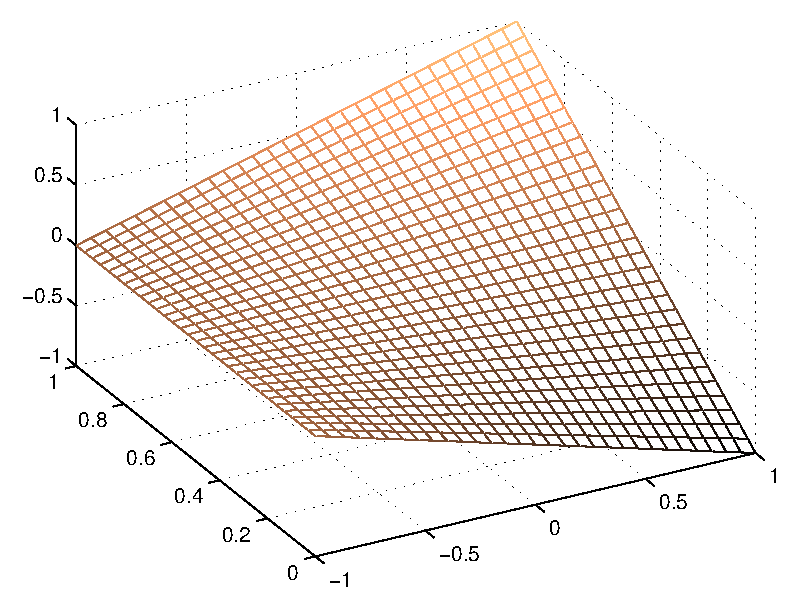
\includegraphics[width=0.4\textwidth]{../figs/tilting_slope_funct3}}
	}
\caption{Two additively unfaithful functions. Relevant variables are
  zeroed out under an additive approximation because every ``slice''
  of the function integrates to zero.}
\vskip-10pt
\end{figure*}


\begin{lemma}
\label{lem:general_int_reduction}
Let $F$ be a product distribution on $\mathbf{C}=[0,1]^s$ with density function $p$ which is positive on $\mathbf{C}$. Let
$X=(X_1,...,X_s) \sim F$. Let $f: \mathbf{C} \rightarrow \R$ be an
integrable function.
Let 
\begin{equation}
\begin{split}
f_k^*, \mu^* \coloneqq \argmin_{f_1,\ldots, f_s, \mu} \Bigl\{ \E \bigl( f(X) & -
 \sum_{k=1}^s f_k(X_k) -\mu \bigr)^2 \\
       & \,:\, \E f_k(X_k) = 0\Bigr\}.
\end{split}
\end{equation}
Then $\mu^* = \E f(X)$ and $f^*_k(x_k) = \E[ f(X) \given x_k] - \E f(X)$ and this solution is unique.
\end{lemma}

Lemma~\ref{lem:general_int_reduction} follows from the stationarity
conditions of the optimal solution. If $F$ is the uniform distribution,
then $f^*_k(x_k) = \int f(x_k, \mathbf{x}_{-k})
d\mathbf{x}_{-k}$.

\begin{example} We give two examples of additive unfaithfulness under
  the uniform distribution. First, consider the following function:
\[
\trm{(egg carton)} \quad f(x_1, x_2) = \sin( 2\pi x_1) \sin( 2 \pi x_2)
\]
defined for $(x_1, x_2) \in [0,1]^2$.  Then
$\int_{x_2} f(x_1, x_2) d x_2 = 0$ and
$\int_{x_1} f(x_1, x_2) d x_1 = 0$ for each $x_1$ and $x_2$. An additive approximation
would set $f_1 = 0$ and $f_2 = 0$.  Next, consider the function
\[
\trm{(tilting slope)} \quad f(x_1, x_2) = x_1 x_2
\]
defined for $x_1 \in [-1,1],\; x_2 \in [0,1]$.  In this case
$\int_{x_1} f(x_1, x_2) d x_1 = 0$ for each $x_2$; therefore, we expect $f_2 = 0$ under the additive approximation. This function, for every fixed $x_2$, is a zero-intercept linear function of $x_1$ with slope $x_2$.
\end{example}

In order to exploit additive models, it is important to understand when the
additive approximation accurately captures all of the relevant variables.
We call this property \emph{additive faithfulness}.

\begin{definition}
  Let $\mathbf{C}=[0,1]^s$, and $f:\mathbf{C}\rightarrow \R$. We say
  that $f$ \emph{depends on} coordinate $k$ if there exist $x'_k \neq
  x_k$ such that $f(x'_k, \mathbf{x}_{-k})$ and $f(x_k,
  \mathbf{x}_{-k})$ are different functions of $\mathbf{x}_{-k}$.

Let $F$ be a probability distribution on $\mathbf{C}$ and
assume without loss of generality that $\E f(X) = 0$. Let 
\begin{equation}
\begin{split}
f_k^*, \mu^* \coloneqq \argmin_{f_1,\ldots, f_s, \mu} \Bigl\{ 
             \E ( f(X) &- \sum_{k=1}^s f_k(X_k) -\mu )^2 \\
         &\,:\, \E f_k(X_k) = 0 \Bigr\}.
\end{split}
\end{equation}
We say that $f$ is \emph{additively faithful} under $F$ in case $f^*_k = 0$ iff $f$ does not depend on coordinate $k$. 
\end{definition}
% We can define the support $\trm{supp}(f) \coloneqq \{ k \,:\,
% \trm{$k$ is relevant to $f$}\}$. Let $f^* = \sum_{k=1}^s$, then $f$
% is additively faith if $\trm{supp}(f) = \trm{supp}(f^*)$.

Remarkably, under product distributions, a convex multivariate function can always be faithfully approximated by an additive function. 

\begin{theorem}
\label{thm:convex_faithful}
Let $F$ be a product distribution supported on $C=[0,1]^s$ with positive density $p$. If $f$ is convex and twice differentiable, then $f$ is additively faithful under $F$.
\end{theorem}

We give the full proof in Section~\ref{sec:faithful_proof} of the
Appendix, but pause here to provide some intuition. From
Lemma~\ref{lem:general_int_reduction}, we know that the
additive approximation zeroes out $k$ when, fixing $x_k$, every
``slice'' of $f$ integrates to zero. We prove
Theorem~\ref{thm:convex_faithful} by showing that ``slices'' of convex
functions that integrate to zero cannot be ``glued'' together while
still maintaining convexity.

Theorem~\ref{thm:convex_faithful} plays an important role in our
sparsistency analysis, where we show that the additive
approximation is variable selection consistent (or ``sparsistent''), even when the true function is not
additive.

\begin{remark}
  We assume twice differentiability in
  Theorem~\ref{thm:convex_faithful} to simplify the proof. We believe
  this smoothness condition is not necessary because every non-smooth
  convex function can be approximated arbitrarily well by a smooth
  one.  
\end{remark}
\begin{remark}
Without restrictions on the distribution, a convex
  function may not be additively faithful. Intuitively, an arbitrarily shaped
  density $p$
  may ``undo'' the convexity of $f$ so that the product
  $p(\mathbf{x}) \, f(\mathbf{x})$ resembles an egg carton or a
  tilting slope.  With appropriate conditions on the density $p$,
  however, it is possible to relax the independence assumption.  We leave this to
  future work.
\end{remark}

\section{Optimization for Sparse Convex Additive Models}

We now consider the following nonparametric regression problem
\begin{equation}\nonumber
          Y_{i} = f(\bds{x}_{i}) + \epsilon_{i} = 
                  \sum_{k=1}^{p}f_{k}(x_{ki}) + \epsilon_{i} \quad i=1,2,\cdots,n
\end{equation}
where $\bds{x}_{i}\in\mathbb{R}^{p}$ is the covariate, $Y_{i}$ is the
response and $\epsilon_{i}$ is mean zero noise. The regression function $f(\cdot)$ is the summation of 
functions $f_{k}(\cdot)$ in each variable dimension.  
We impose an additional constraint that each $f_{k}(\cdot)$ is 
an univariate convex function, which can be represented by its supporting hyperplanes, i.e.,
\begin{equation}\label{hyper}
      h_{kj} \geq h_{ki} + \beta_{ki}(x_{kj}-x_{ki}) \quad (\forall i,j)
\end{equation}
where $h_{ki}\coloneqq f_{k}(x_{ki})$ and $\beta_{ki}$ is the
subgradient at point $x_{ki}$. We apparently need $O(n^2 p)$ constraints to
impose the supporting hyperplane constraints, which is computationally
expensive for large scale problems.  In fact, only $O(np)$
constraints suffice, since univariate convex functions are
characterized by the condition that the subgradient, which is a scalar, must
increase monotonically. This observation leads to our optimization
program:
\begin{equation}\begin{split}\label{np}
       &\min_{\bds{h},\bds{\beta},\mu} \ \frac{1}{2n}\sum_{i=1}^{n}
                     \Bigl( Y_{i}-\sum_{k=1}^{p}h_{ki} - \mu \Bigr)^{2} 
                         + \lambda\sum_{k=1}^{p}\|\bds{\beta}_{k\cdot}\|_{\infty} \\
       &\ \textrm{s.t.} \ \sum_{i=1}^{n}h_{ki}=0,\; h_{k(i+1)} = h_{k(i)} + \beta_{k(i)}(x_{k(i+1)}-x_{k(i)}), 
                                 \ \beta_{k(i+1)} \geq \beta_{k(i)} \ (\forall k, i)
\end{split}\end{equation}
We introduce a mean parameter $\mu \in \R$ because $f$ may not have zero-mean. We can in fact solve $\mu$ explicitly here: the optimal $\mu = \frac{1}{n} \sum_{i=1}^n Y_i = \bar{Y}$ because of KKT and the constraints that $\sum_i h_{ki} = 0$.
$\{(1),(2),\ldots,(n)\}$ is a reordering of $\{1,2,\ldots,n\}$ such that $x_{k(1)}\leq{}x_{k(2)}\leq\cdots\leq{}x_{k(n)}$.  It is easy to verify that the constraints in (\ref{np}) satisfy the supporting hyperplane constraints, as
\begin{align*}
  \forall j\geq{}i, &h_{k(j)}-h_{k(i)}  = 
            \sum\limits_{t=i}^{j-1}(h_{k(t+1)}-h_{k(t)}) = 
            \sum\limits_{t=i}^{j-1}\beta_{k(t)}(x_{k(t+1)}-x_{k(t)})\\ 
      & \geq \beta_{k(i)}\sum\limits_{t=i}^{j-1}(x_{k(t+1)}-x_{k(t)}) = \beta_{k(i)}(x_{k(j)}-x_{k(i)}) \\
  \forall j<i, &h_{k(j)}-h_{k(i)} =
                \sum\limits_{t=j}^{i-1}(h_{k(t)}-h_{k(t+1)}) = 
                \sum\limits_{t=j}^{i-1}\beta_{k(t)}(x_{k(t)}-x_{k(t+1)}) \\ 
     & \geq \beta_{k(i)}\sum\limits_{t=j}^{i-1}(x_{k(t)}-x_{k(t+1)}) = \beta_{k(i)}(x_{k(j)}-x_{k(i)}), 
\end{align*}
The $\ell_\infty/\ell_1$ penalty
$\sum_{k=1}^{p}\|\bds{\beta}_{k\cdot}\|_{\infty}$ encourages group
sparsity of the vectors $\bds{\beta}_{k\cdot}$, and thus performs
variable selection.  We refer to this framework as the sparse convex
additive model (SCAM). Notice that if we replace $\beta_{k(i+1)} \geq
\beta_{k(i)}$ with $\beta_{k(i+1)}=\beta_{k(i)}$, the optimization
reduces to the lasso.  Note while one can use
supporting hyperplanes to the epigraph as in \eqref{eq:outer}, 
SCAM uses the \emph{inner  piece-wise linear function}
that approximates the graph with secant lines.


%\begin{SCfigure}
%\label{fig:outer_approximation}
%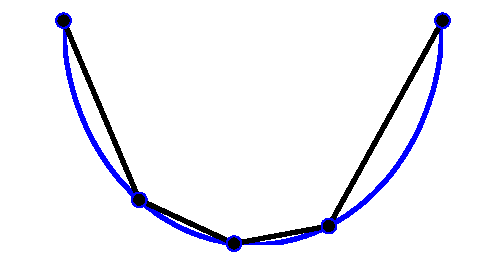
\includegraphics[width=0.3\textwidth]{figs/outer_approximation.pdf}
%\caption{With the 5 sample points $(X_i, h(X_i))$, the
%  black and the blue convex function represent equivalent fits. SCAM
%  chooses the inner piece-wise linear convex functions.}
%\end{SCfigure}

The SCAM optimization in (\ref{np}) is a quadratic program (QP) with $O(np)$ variables and $O(np)$ constraints. The optimal $\mu$ has a closed form solution of $\mu = \frac{1}{n}\sum_{i=1}^n Y_i$, which is easy to derive from the KKT theorem and the constraints that $\sum_i h_{ki} = 0$ for all $k$.
Directly applying a QP solver for $\bds{h}, \bds{\beta}$ would be computationally expensive for relatively large $n$ and $p$. However, notice that variables
in different feature dimensions are only coupled in the term $(Y_{i}-\sum_{k=1}^{p}h_{ki})^{2}$. Hence, we can apply the block coordinate descent method,
where in each step we solve the following QP subproblem for
$\{\bds{h}_{k\cdot},\bds{\beta}_{k\cdot}\}$ with the other variables fixed:
\begin{equation}\begin{split}\nonumber
       &\min_{\bds{h}_{k\cdot},\bds{\beta}_{k\cdot},\gamma_{k}} 
             \ \frac{1}{2n}\sum_{i=1}^{n}\Bigl((Y_{i}-\bar{Y}-\sum_{r\neq{k}}h_{ri})-h_{ki}\Bigr)^{2} 
                      + \lambda\gamma_{k} \\
        &\ \textrm{s.t.} \ \sum_{i=1}^{n}h_{ki}=0, \ h_{k(i+1)} = h_{k(i)} + \beta_{k(i)}(x_{k(i+1)}-x_{k(i)}), \ \beta_{k(i+1)} \geq \beta_{k(i)}, \ -\gamma_{k}\leq\beta_{k(i)}\leq\gamma_{k} \ (\forall i).
\end{split}\end{equation}
The extra variable $\gamma_{k}$ is introduced to deal with the $\ell_{\infty}$ norm. This QP subproblem involves $O(n)$ variables, $O(n)$ constraints and a sparse structure, 
which can be solved efficiently using optimization packages (e.g., MOSEK: \verb+http://www.mosek.com/+).  We cycle through all feature dimensions ($k$) from $1$ to $p$ multiple times until convergence.
Empirically, we observe that the algorithm converges in only a few cycles. We also implemented an ADMM solver for (\ref{np}), but found that it is not as efficient as this QP solver.

After optimization, the function estimator for any input data $\bds{x}_j$ is, according to (\ref{hyper}),
\begin{equation}\nonumber
      f(\bds{x}_j) = \sum_{k=1}^{p}f_k(x_{kj})+\mu = \sum_{k=1}^{p}\max_{i} \{h_{ki}+\beta_{ki}(x_{kj}-x_{ki})\} + \mu.
\end{equation} 


\subsection{Alternative Formulation}
Optimization (\ref{np}) can be reformulated in terms of the 2nd derivatives. The alternative formulation replaces the ordering
constraints $\beta_{k(i+1)} \geq \beta_{k(i)}$ with positivity
constraints, which simplifies theoretical analysis.
Define $d_{k(i)}$ as the second derivative:
$d_{k(1)} = \beta_{k(1)}$, and $d_{k(2)} =
\beta_{k(2)} - \beta_{k(1)}$. The convexity constraint is
equivalent to the constraint that $d_{k(i)} \geq 0$ for all $i >
1$.

It is easy to verify that $\beta_{k(i)} = \sum_{j \leq i} d_{k(i)}$ and 
\[
f_k(x_{k(i)}) = f_k({x_{k(1)}}) +d_{k(1)} ( x_{k(i)}
- x_{k(1)}) + d_{k(2)} ( x_{k(i)} - x_{k(2)}) + \cdots + d_{k(i-1)} ( x_{k(i)} - x_{k(i-1)})
\]
We can write this more compactly in matrix notations. First define $\Delta_{k(j)}(x_{ki}) = \max( x_{ki} - x_{k(j)}, 0)$. 
\[
\left[ \begin{array}{c}
    f_k(x_{k1}) \\
    ... \\
    f_k(x_{kn}) \\
\end{array} \right] =
\left[ \begin{array}{ccc}
    \Delta_{k(1)}(x_{k1}) & ... & \Delta_{k(n-1)}(x_{k1}) \\
    ... & & \\
    \Delta_{k(1)}(x_{kn}) & ... & \Delta_{k(n-1)}(x_{kn}) 
\end{array} \right]
\left[ \begin{array}{c}
    d_{k(1)} \\
    ... \\
    d_{k(n-1)}
\end{array} \right] \coloneqq \Delta_k d_k
\]
Where $\Delta_k$ is a $n\times n-1$ matrix such that $\Delta_k(i,j) = \Delta_{k(j)}(x_{k(i)})$ and $d_k = (d_{k(1)} ,..., d_{k(n-1)})$. We can now reformulate (\ref{np}) as an equivalent optimization program with only centering and positivity constraints:
\begin{align}
\min_{d_k \in \R^{n-1}, c_k \in \R,\mu \in \R}& \frac{1}{2n} 
       \Bigl\| Y - \bar{Y}\mathbf{1}_n - \sum_{k=1}^p ( \Delta_k d_k - c_k \mathbf{1}_n) \Bigr\|_2^2 
               + \lambda_n \sum_{k=1}^p \|d_k\|_1  & \label{opt:alternate_opt} \\
\trm{s.t. $\forall k$, }  & d_{k(2)}, \ldots , d_{k(n-1)} \geq 0 	
               \qquad &\trm{(convexity)} \nonumber \\ 
	& c_k = \frac{1}{n} \mathbf{1}_n^\tran \Delta_k d_k 	
               \qquad &\trm{(centering)} \nonumber 
\end{align}
$\|d_k\|_1$ is not identical to $\|\bds{\beta}_{k\cdot}\|_{\infty}$, but it is easy to verify that $\|\bds{\beta}_{k\cdot}\|_{\infty} \leq \|d_k\|_1 \leq 2\|\bds{\beta}_{k\cdot}\|_{\infty}$.

\begin{remark}
\label{rem:bounded_lipschitz_constraints}
For parts of our theoretical analysis, we will also impose onto (\ref{opt:alternate_opt}) a boundedness constraint $-B \mathbf{1}_n \leq \Delta_k d_k + c_k \mathbf{1}_n \leq B \mathbf{1}_n$ which constrains that $\|f_k \|_\infty \leq B$, or a Lipschitz constraint $\|d_k\|_1 \leq L$ which constrains that $f_k$ must be $L$-Lipschitz. We use these constraints only in the proof for technical reasons; we never need nor use these constraints in our experiments.
\end{remark}



\section{Analysis of Variable Selection Consistency}

We divide our analysis into two parts. We first establish a sufficient
\emph{deterministic} condition for sparsistency.  We then consider the
stochastic setting and argue that the deterministic conditions hold with high probability. 

\subsection{Deterministic Setting}

We follow \cite{Wain:09a} and define the \emph{restricted regression} purely for theoretical purposes.
\begin{definition}
In \emph{restricted regression}, we restrict the indices $k$ in
optimization (\ref{opt:alternate_opt}) to lie in the support $S$ instead of ranging from $1,...,p$. 
\end{definition}

Our analysis then differs from the now-standard ``primal-dual witness
technique''~\cite{Wain:09a}. Primal-dual witness explicitly solves all the dual variables, but because our optimization is more complex, we do not solve the dual variables on $S$; we instead write the dual variables on $S^c$ as a function of the restricted regression \emph{residual}, which is implicitly a function of the dual variables on $S$.

\begin{theorem} (Deterministic setting)
\label{thm:deterministic}
Let $\{\hat{d}_k, \hat{c}_k\}_{k \in S}$ be the minimizer of the restricted regression, that is, the solution to optimization (\ref{opt:alternate_opt}) where we restrict $k \in S$. Let $\hat{d}_k = 0$ and $ \hat{c}_k = 0$ for $k \in S^c$.
Let $\hat{r} \coloneqq Y - \bar{Y}\mathbf{1}_n - \sum_{k \in S} (\Delta_k \hat{d}_k -
\hat{c}_k \mathbf{1}_n)$ be the restricted regression residual. For $k
\in \{1,...,p\}$, Let $\Delta_{k, j} \in R^n$ be the $j$-th column of $\Delta_k$, i.e. $\max( X_k - X_{k (j)} \mathbf{1}_n, 0)$. \\

Suppose for all $j$ and all $k\in S^c$, $\lambda_n > | \frac{1}{n}
\hat{r}^\tran \Delta_{k,j}|$. Then $\hat{\mu}$ and $\hat{d}_k, \hat{c}_k$ for $k=1,...,p$ is an optimal solution to the full regression \ref{opt:alternate_opt}. Furthermore, any solution to the optimization program \ref{opt:alternate_opt} must be zero on $S^c$.
\end{theorem}

This result holds regardless of whether we impose the boundedness and Lipschitz conditions in optimization~\ref{opt:alternate_opt}.
The full proof of Theorem~\ref{thm:deterministic} is in Section~\ref{sec:deterministic_proof} of the Appendix.

\begin{remark}
  The incoherence condition of \cite{Wain:09a} is implicitly encoded
  in our condition on $\lambda_n, \hat{r}, \Delta_{k,j}$. We can
  reconstruct the incoherence condition if we assume that the true
  function $f_0$ is linear and that our fitted functions $\hat{f}_k$
  are linear as well.
\end{remark}

Theorem~\ref{thm:deterministic} allows us to analyze false negative
rates and false positive rates separately. To control false positives,
we study when the condition $\lambda_n > | \frac{1}{n} \hat{r}^\tran
\Delta_{k,j}|$ is fulfilled for all $j$ and all $k \in S^c$. To
control false negatives, we study the restricted regression.

\subsection{Probabilistic Setting}

We use the following statistical setting:

\begin{packed_enum}
\item Let $F$ be a distribution supported and positive on $\mathcal{X}=[-b,b]^p$. Let $X^{(1)},..., X^{(n)} \sim F$ be iid.
\item Let $Y = f_0(X) + \epsilon$ where $\epsilon$ is zero-mean noise. Let $Y^{(1)},...,Y^{(n)}$ be iid.
\item Let $S = \{1,...,s\}$ denote the relevant variables where $s\leq p$, i.e.,
  $f_0(X) = f_0(X_S)$.
\item Let $f^*_1,...,f^*_s \coloneqq \argmin_{f_1,...,f_s} \{ \E(f_0(X) - \sum_{k=1}^s f_k(X_k))^2 \,|\, \E[f_k(X_k)] = 0 \}$.
\end{packed_enum}

Each of our theorems will use a subset of the following assumptions:
\begin{packed_enum}
\item[A1:] $X_S, X_{S^c}$ are independent.  \ A1': $\{ X_k \}_{k \in S}$ are independent.
\item[A2:] $\|f_0\|_\infty \leq sB$ \  A2': $f_0$ is convex,
  twice-differentiable, $L$-Lipschitz, and $\trm{supp}(f_0) = S$.
\item[A3:] Suppose $\epsilon$ is mean-zero sub-Gaussian, independent of $X$, with sub-Gaussian scale $\sigma$, i.e. for all $t \in \R$, $\E e^{t \epsilon} \leq \E e^{\sigma^2 t^2 / 2}$.
\item[A4:] For all $k=1,...,s$, $\E(f^*_s(X_k))^2 \geq \alpha$ for some positive constant $\alpha$.
\end{packed_enum}

We will use assumptions A1, A2, A3 to control the probability of false
positives and the stronger assumptions A1', A2', A3, A4 to control the
probability of false negatives.  Assumption A4 can be
weakened so that the relevant functions satisfy
$\E(f^*_s(X_k))^2 \geq \alpha_n$ for $\alpha_n$ decaying to zero 
at an appropriate rate.



\begin{remark}
  We make strong assumptions on the covariates in A1 in order to make
  very weak assumptions on the true regression function $f_0$ in
  A2. In particular, we do not assume that $f_0$ is additive. Relaxing
  these assumptions is an interesting direction for future work. 
  %Strong assumptions on the covariates are not uncommon in nonparametric
  %variable selection analysis~\cite{lafferty2008rodeo}. 
  %[TODO: refer to correlated design experiment].
\end{remark}

\begin{remark}
Assumption A4 ensures that the relevant variables are ``relevant enough''. Under A4, the population risk of an additive function with $s-1$ components is at least $\alpha$ larger than the population risk of the optimal additive function with $s$ components. Lemma~\ref{lem:minus_one_risk_increase} in section~\ref{sec:false_negative_proof} of the appendix.
\end{remark}

\begin{theorem} (Controlling false positives) 
\label{thm:false_positive}
Suppose assumptions A1, A2, A3 hold. Suppose also that we run optimization~\eqref{opt:alternate_opt} with the $B$-boundness constraint. Let $c,C$ be absolute constants.
Suppose $\lambda_n \geq c b (sB + \sigma) \sqrt{ \frac{s}{n} \log n
  \log (pn)}$.  Then with probability at least $ 1 - \frac{C}{n}$, for all $j,k$, $\lambda_n >  | \frac{1}{n} \hat{r}^\tran \Delta_{k,j}|$.
Therefore, any solution to the full regression (\ref{opt:alternate_opt}), with boundedness constraint, is zero on $S^c$. 
\end{theorem}

The proof of Theorem~\ref{thm:false_positive} exploits independence of
$\hat{r}$ and $\Delta_{k,j}$ from A1, and then uses concentration of
measure results to argue that $| \frac{1}{n} \hat{r}^\tran
\Delta_{k,j}|$ concentrates around zero at a desired rate. The fact
that $\hat{r}$ is a centered vector is crucial to our proof, and our
theory thus further illustrates the importance of imposing the
centering constraints in optimization \eqref{opt:alternate_opt}. Our
proof uses the concentration of the average of
data sampled \emph{without} replacement
\cite{serfling1974probability}, illustrating that the proof method is not a
trivial application of existing techniques. The full proof of
Theorem~\ref{thm:false_positive} is in
Section~\ref{sec:false_positive_proof} of the Appendix.

\begin{theorem} (Controlling false negatives)
\label{thm:false_negative}
Suppose assumptions A1', A2', A3, A4 hold. Let $\ds \hat{f} = \{ \hat{d}_k, \hat{c}_k\}_{k\in S}$ be any solution to the restricted regression with both the $B$-boundedness and $L$-Lipschitz constraint. Let $c,C$ be absolute constants.
Suppose $s L \lambda_n \rightarrow 0$ and $bL (B+\sigma)B\sigma \sqrt{\frac{s^5}{n^{4/5}} \log sn} \rightarrow 0$.
Then, for sufficiently large $n$, $\hat{f}_k = (\hat{d}_k, \hat{c}_k)
\neq 0$ for all $k \in S$ with probability at least $1-\frac{C}{n}$.
\end{theorem}

This is a finite sample version of
Theorem~\ref{thm:convex_faithful}. We need stronger assumptions in
Theorem~\ref{thm:false_negative} to use our additive faithfulness
result, Theorem~\ref{thm:convex_faithful}. We also include an extra
Lipschitz constraint so that we can use existing covering number
results \cite{Bronshtein:76}. Recent work
\cite{Guntu:13} shows that the Lipschitz constraint
is not required with more advanced empirical process theory
techniques. We give the full proof of Theorem~\ref{thm:false_negative}
in Section~\ref{sec:false_negative_proof} of the Appendix.

Combining Theorem~\ref{thm:false_positive} and
~\ref{thm:false_negative} and ignoring dependencies on $b,B,L,\sigma$,
we have the following result.
\begin{corollary}
  Assume A1', A2', A3, A4. Let $\lambda_n = \Theta\left( \sqrt{
  \frac{s^3}{n} \log n \log (pn)} \right)$. Suppose $s \lambda_n
  \rightarrow 0$ and $\sqrt{\frac{s^5}{n^{4/5}} \log sn} \rightarrow
  0$. Let $\hat{f_n}$ be a solution to (\ref{opt:alternate_opt}) with
  boundedness and Lipschitz constraints. Then 
  $\P( \trm{supp}(\hat{f_n}) = \trm{supp}(f_0) ) \rightarrow 1$.
\end{corollary}
The above corollary implies that sparsistency is achievable at the same exponential scaling of the ambient dimension $p = O(\exp(n^c)), c<1$ rate as parametric models. The cost of nonparametric modeling is reflected in the scaling with respect to $s$, which can only scale at $o(n^{4/25})$.

%\textbf{Comparison with Related Work.} 


% DO NOT CHANGE; RefTex variables -minx
 
%%% Local Variables: ***
%%% mode:latex ***
%%% TeX-master: "scam_icml.tex" ***
%%% End: ***

\section{Experiments}
%\subsection{Simulations}
We first illustrate our methods using a simulation of the following regression problem
\begin{equation}\nonumber
         y_i = \bds{x}_{iS}^{\top}\bds{Q}\bds{x}_{iS} + \epsilon_i \quad (i=1,2,\ldots,n).
\end{equation}
Here $\bds{x}_{i}$ denotes data sample $i$ drawn from $\mathcal{N}(\bds{0},\bds{I}_{p})$, 
$\bds{x}_{iS}$ is a subset of $\bds{x}_i$ with dimension $|S|=5$, where $S$ represents the active feature set, and 
$\epsilon_i$ is the additive noise drawn from $\mathcal{N}(0,1)$. 
$\bds{Q}$ is a symmetric positive definite matrix of dimension $|S|\times{}|S|$. 
Notice that if $\bds{Q}$ is diagonal, then the true function is convex additive; otherwise the true function is convex but not additive.
For all the simulations in this section, we set $\lambda=4\sqrt{{\log(np)}/{n}}$.

In the first simulation, we set $\bds{Q}=\bds{I}_{|S|}$ (the additive
case), and choose $n=100, 200,\ldots,1000$ and $p=64,128,256,512$.
For each $(n,p)$ combination, we generate $200$ independent data
sets. For each data set we use SCAM to infer the model parameterized
by $\bds{h}$ and $\bds{\beta}$; see equation \eqref{np}. If
$\|\bds{\beta}_{k\cdot}\|_{\infty}<10^{-8}\ (\forall k\not\in{}S)$ and
$\|\bds{\beta}_{k\cdot}\|_{\infty}>10^{-8}\ (\forall k\in{}S)$, then
we declare correct support recovery. We then plot the probability of
support recovery over the $200$ data sets in Figure \ref{Support}(a).  We
observe that SCAM performs consistent variable selection when the true
function is convex additive.  
To give the reader a
sense of the running speed, the code runs in about $2$ minutes on one
data set with $n=1000$ and $p=512$, on a MacBook with 2.3 GHz Intel
Core i5 CPU and 4 GB memory.

In the second simulation, we study the case in which the true function
is convex but not additive. We generate four $\bds{Q}$ matrices
plotted in Figure \ref{Support}(b), where the diagonal elements are all $1$ and
the off-diagonal elements are $0.5$ with probability $\alpha$
($\alpha=0,0.2,0.5,1$ for the four cases). We fix $p=128$ and choose
$n=100,200,\ldots,1000$. We again run the SCAM optimization on $200$
independently generated data sets and plot the probability of recovery
in Figure \ref{Support}(c). The results demonstrate that SCAM performs
consistent variable selection even if the true function is not additive (but
still convex).

In the third simulation, we study the case of correlated design, where
$\bds{x}_{i}$ is drawn from $\mathcal{N}(\bds{0},\bds{\Sigma})$
instead of $\mathcal{N}(\bds{0},\bds{I}_{p})$, with
$\Sigma_{ij}=\nu^{|i-j|}$. We use the non-additive $\bds{Q}$ with
$\alpha=0.5$ and fix $p=128$.  The recovery curves for $\nu=02, 0.4,
0.6, 0.8$ are depicted in Figure \ref{Support}(d). As can be seen, for
design of moderate correlation, SCAM can still select relevant
variables well.


%\begin{figure}[!htpb]
%        \centering
%        \begin{subfigure}[b]{0.45\textwidth}
%                \centering
%                \includegraphics[width=\textwidth]{figs/Curve1}
%                 \caption{Additive model.}
%                \label{Curve1}
%        \end{subfigure}
%        \begin{subfigure}[b]{0.45\textwidth}
%                \centering
%                \includegraphics[width=\textwidth]{figs/Q}
%                \caption{Four $\bds{Q}$ matrices.}
%                \label{Q}
%        \end{subfigure}\\
%        \begin{subfigure}[b]{0.45\textwidth}
%                \centering
%                \includegraphics[width=\textwidth]{figs/Curve2}
%                \caption{Additive and non-additive models.}
%                \label{Curve2}
%        \end{subfigure}
%        \begin{subfigure}[b]{0.45\textwidth}
%                \centering
%                \includegraphics[width=\textwidth]{figs/Curve3}
%                \caption{Correlated design for non-additive model.}
%                \label{Curve3}
%        \end{subfigure}
%        \caption{Result of support recovery.}\label{Support}
%\end{figure}

%\begin{figure}[ht]
%\begin{center}
%\begin{tabular}{cccc}
%\hskip-20pt
%\includegraphics[width=.27\textwidth]{figs/Curve1} &
%\hskip-17pt
%\includegraphics[width=.27\textwidth]{figs/Q} &
%\hskip-17pt
%\includegraphics[width=.27\textwidth]{figs/Curve2} &
%\hskip-17pt
%\includegraphics[width=.27\textwidth]{figs/Curve3}  \\
%(a) additive model & (b) four $\bds{Q}$ matrices &
%(c) non-additive models & (d) correlated design
%\end{tabular}
%\end{center}
%\caption{Result of support recovery.}\label{Support}
%\end{figure}


%\subsection{Boston housing data}

We next use the Boston housing data rather than simulated data. This data set
contains 13 covariates, 506 samples and one response variable
indicating housing values in suburbs of Boston. The data and detailed description
can be found on the UCI Machine Learning Repository website~\verb+http://archive.ics.uci.edu/ml/datasets/Housing+. 

We first use all $n=506$ samples (with normalization) to train SCAM, using
a set of candidate $\{\lambda^{(t)}\}$ with $\lambda^{(1)}=0$ (no regularization). For each $\lambda^{(t)}$
we obtain a subgradient matrix $\bds{\beta}^{(t)}$ with $p=13$ rows. The non-zero
rows in this matrix indicate the variables selected using $\lambda^{(t)}$. 
We plot $\|\bds{\beta}^{(t)}\|_{\infty}$ and the row-wise mean of $\bds{\beta}^{(t)}$ versus the normalized
norm $\frac{\|\bds{\beta}^{(t)}\|_{\infty,1}}{\|\bds{\beta}^{(1)}\|_{\infty,1}}$ in Figures \ref{Boston}(a) and \ref{Boston}(b).
As a comparison we plot the LASSO/LARS result in a similar way in Figure \ref{Boston}(c).
From the figures we observe that the first three variables selected by SCAM
and LASSO are the same: LSTAT, RM and PTRATIO, which is consistent with previous findings~\cite{SpAM:07}.
The fourth variable selected by SCAM is TAX (with $\lambda^{(t)}=0.09$).
We then refit SCAM with only these four variables without regularization, and plot the inferred additive
functions in Figure \ref{Boston}(e). As can be seen, these functions contain clear nonlinear effects which cannot be captured
by LASSO. The shapes of these functions are in agreement with those obtained by SpAM~\cite{SpAM:07}.

Next, in order to quantitatively study the predictive performance, we run 10 times 5-fold cross validation, following
the same procedure described above (training, variable selection and
refitting).  A plot of the mean and standard
deviation of the predictive Mean Squared Error (MSE) in in Figure \ref{Boston}(d). Since for SCAM the same $\lambda^{(t)}$ may lead to
slightly different number of selected features in different folds and runs, the values on the x-axis (average number of selected features)
for SCAM are not necessarily integers. Nevertheless, the figure clearly shows that SCAM has a much lower predictive MSE than LASSO. 
We also compared the performance of SCAM with that of Additive Forward Regression (AFR) presented in~\cite{Xi:09}, and found that they are similar.
The main advantages of SCAM compared with AFR and SpAM are 1) there are no other tuning parameters (such as bandwidth)
besides $\lambda$; 2) SCAM is formulated as a convex program, which guarantees a global optimum.

%\begin{figure}[!htpb]
%        \centering
%        \begin{subfigure}[b]{0.45\textwidth}
%                \centering
%                \includegraphics[width=\textwidth]{figs/Additive}
%                 \caption{Variable selection result using SCAM.}
%                \label{SCAM}
%        \end{subfigure}
%        \begin{subfigure}[b]{0.45\textwidth}
%                \centering
%                \includegraphics[width=\textwidth]{figs/Additive1}
%                 \caption{Variable selection result using SCAM.}
%                \label{SCAM1}
%        \end{subfigure}\\
%        \begin{subfigure}[b]{0.45\textwidth}
%                \centering
%                \includegraphics[width=\textwidth]{figs/LASSO}
%                \caption{Variable selection result using LASSO.}
%                \label{LASSO}
%        \end{subfigure}
%        \begin{subfigure}[b]{0.45\textwidth}
%                \centering
%                \includegraphics[width=\textwidth]{figs/MSE}
%                 \caption{Predictive MSE of SCAM and LASSO.}
%                 \label{MSE}
%        \end{subfigure}\\
%        \begin{subfigure}[b]{0.45\textwidth}
%                \centering
%                \includegraphics[width=\textwidth]{figs/Convex}
%                \caption{Inferred additive convex functions by SCAM.}
%                \label{Convex}
%        \end{subfigure}
%        \caption{Results on Boston housing data.}\label{Boston}
%\end{figure}


\begin{figure*}[!t]
\begin{center}
\begin{tabular}{cccc}
\hskip-20pt
\includegraphics[width=.29\textwidth]{../figs/Curve1} &
\hskip-20pt
\includegraphics[width=.29\textwidth]{../figs/Q} &
\hskip-20pt
\includegraphics[width=.29\textwidth]{../figs/Curve2} &
\hskip-20pt
\includegraphics[width=.29\textwidth]{../figs/Curve3}  \\
\hskip-10pt (a) additive model & 
\hskip-10pt (b) four $\bds{Q}$ matrices &
\hskip-10pt (c) non-additive models & 
\hskip-10pt (d) correlated design
\end{tabular}
\end{center}
\caption{Support recovery results where the additive assumption is
  correct (a), incorrect (b), (c), and with correlated design (d).}\label{Support}
\vskip10pt

\begin{center}
\begin{tabular}{ccc}
\hskip-10pt
  \includegraphics[width=.35\textwidth]{../figs/Additive} &
\hskip-25pt
  \includegraphics[width=.35\textwidth]{../figs/Additive1} &
\hskip-25pt
  \includegraphics[width=.35\textwidth]{../figs/LASSO} 
\\
\hskip-10pt 
SCAM $\|\beta_k\|_\infty$ paths & 
\hskip-25pt 
SCAM $\text{mean}(\beta_k)$ paths &
\hskip-25pt
LASSO $\beta_k$ paths
\end{tabular}
\begin{tabular}{cc}
  \includegraphics[width=.37\textwidth]{../figs/MSE} &
  \includegraphics[width=.43\textwidth]{../figs/Convex}
\\
predictive MSE & inferred functions from SCAM
\end{tabular}
\end{center}
\caption{Results on Boston housing data, showing regularization paths,
 MSE and fitted functions.}\label{Boston}
\end{figure*}

\section{Discussion}

We have introduced a framework for estimating high dimensional but
sparse convex functions.  Because of the special properties of
convexity, variable selection for convex functions enjoys additive
faithfulness---it suffices to carry out variable selection over an
additive model, in spite of the approximation error this introduces.
Sparse convex additive models can be optimized using block coordinate
quadratic programming, which we have found to be effective and
scalable.  We established variable selection consistency results,
allowing exponential scaling in the ambient dimension.  We expect
that the technical assumptions we have used in these analyses can be
weakened; this is one direction for future work.  Another interesting
direction for building on this work is to allow for additive models that
are a combination of convex and concave components.  If the
convexity/concavity of each component function is known, this again
yields a convex program.  The challenge is to develop a method to
automatically detect the concavity or convexity pattern of the
variables.




\newpage
\bibliography{local}
\bibliographystyle{icml2014}

\newpage
\onecolumn{
\input{appendix_icml.tex}
}
\end{document} 


% This document was modified from the file originally made available by
% Pat Langley and Andrea Danyluk for ICML-2K. This version was
% created by Lise Getoor and Tobias Scheffer, it was slightly modified  
% from the 2010 version by Thorsten Joachims & Johannes Fuernkranz, 
% slightly modified from the 2009 version by Kiri Wagstaff and 
% Sam Roweis's 2008 version, which is slightly modified from 
% Prasad Tadepalli's 2007 version which is a lightly 
% changed version of the previous year's version by Andrew Moore, 
% which was in turn edited from those of Kristian Kersting and 
% Codrina Lauth. Alex Smola contributed to the algorithmic style files.  
